\subsection{Accorgimenti}

\paragraph{Angoli}
\label{spiegazione}

Nel posizionare il coperchio della camera a vuoto c'è un gioco dell'ordine di \SI{1}{\degree}.
Eliminiamo questa sistematica spingendo sempre verso un certo lato il coperchio quando chiudiamo la camera;
una volta fatto il vuoto la pressione atmosferica blocca saldamente il coperchio.
Riduciamo la parallasse nella lettura degli angoli
attaccando un pezzo di carta con una tacca al supporto della sorgente (vedi \autoref{fig:parallasse}).

\begin{figure}
	\centering
	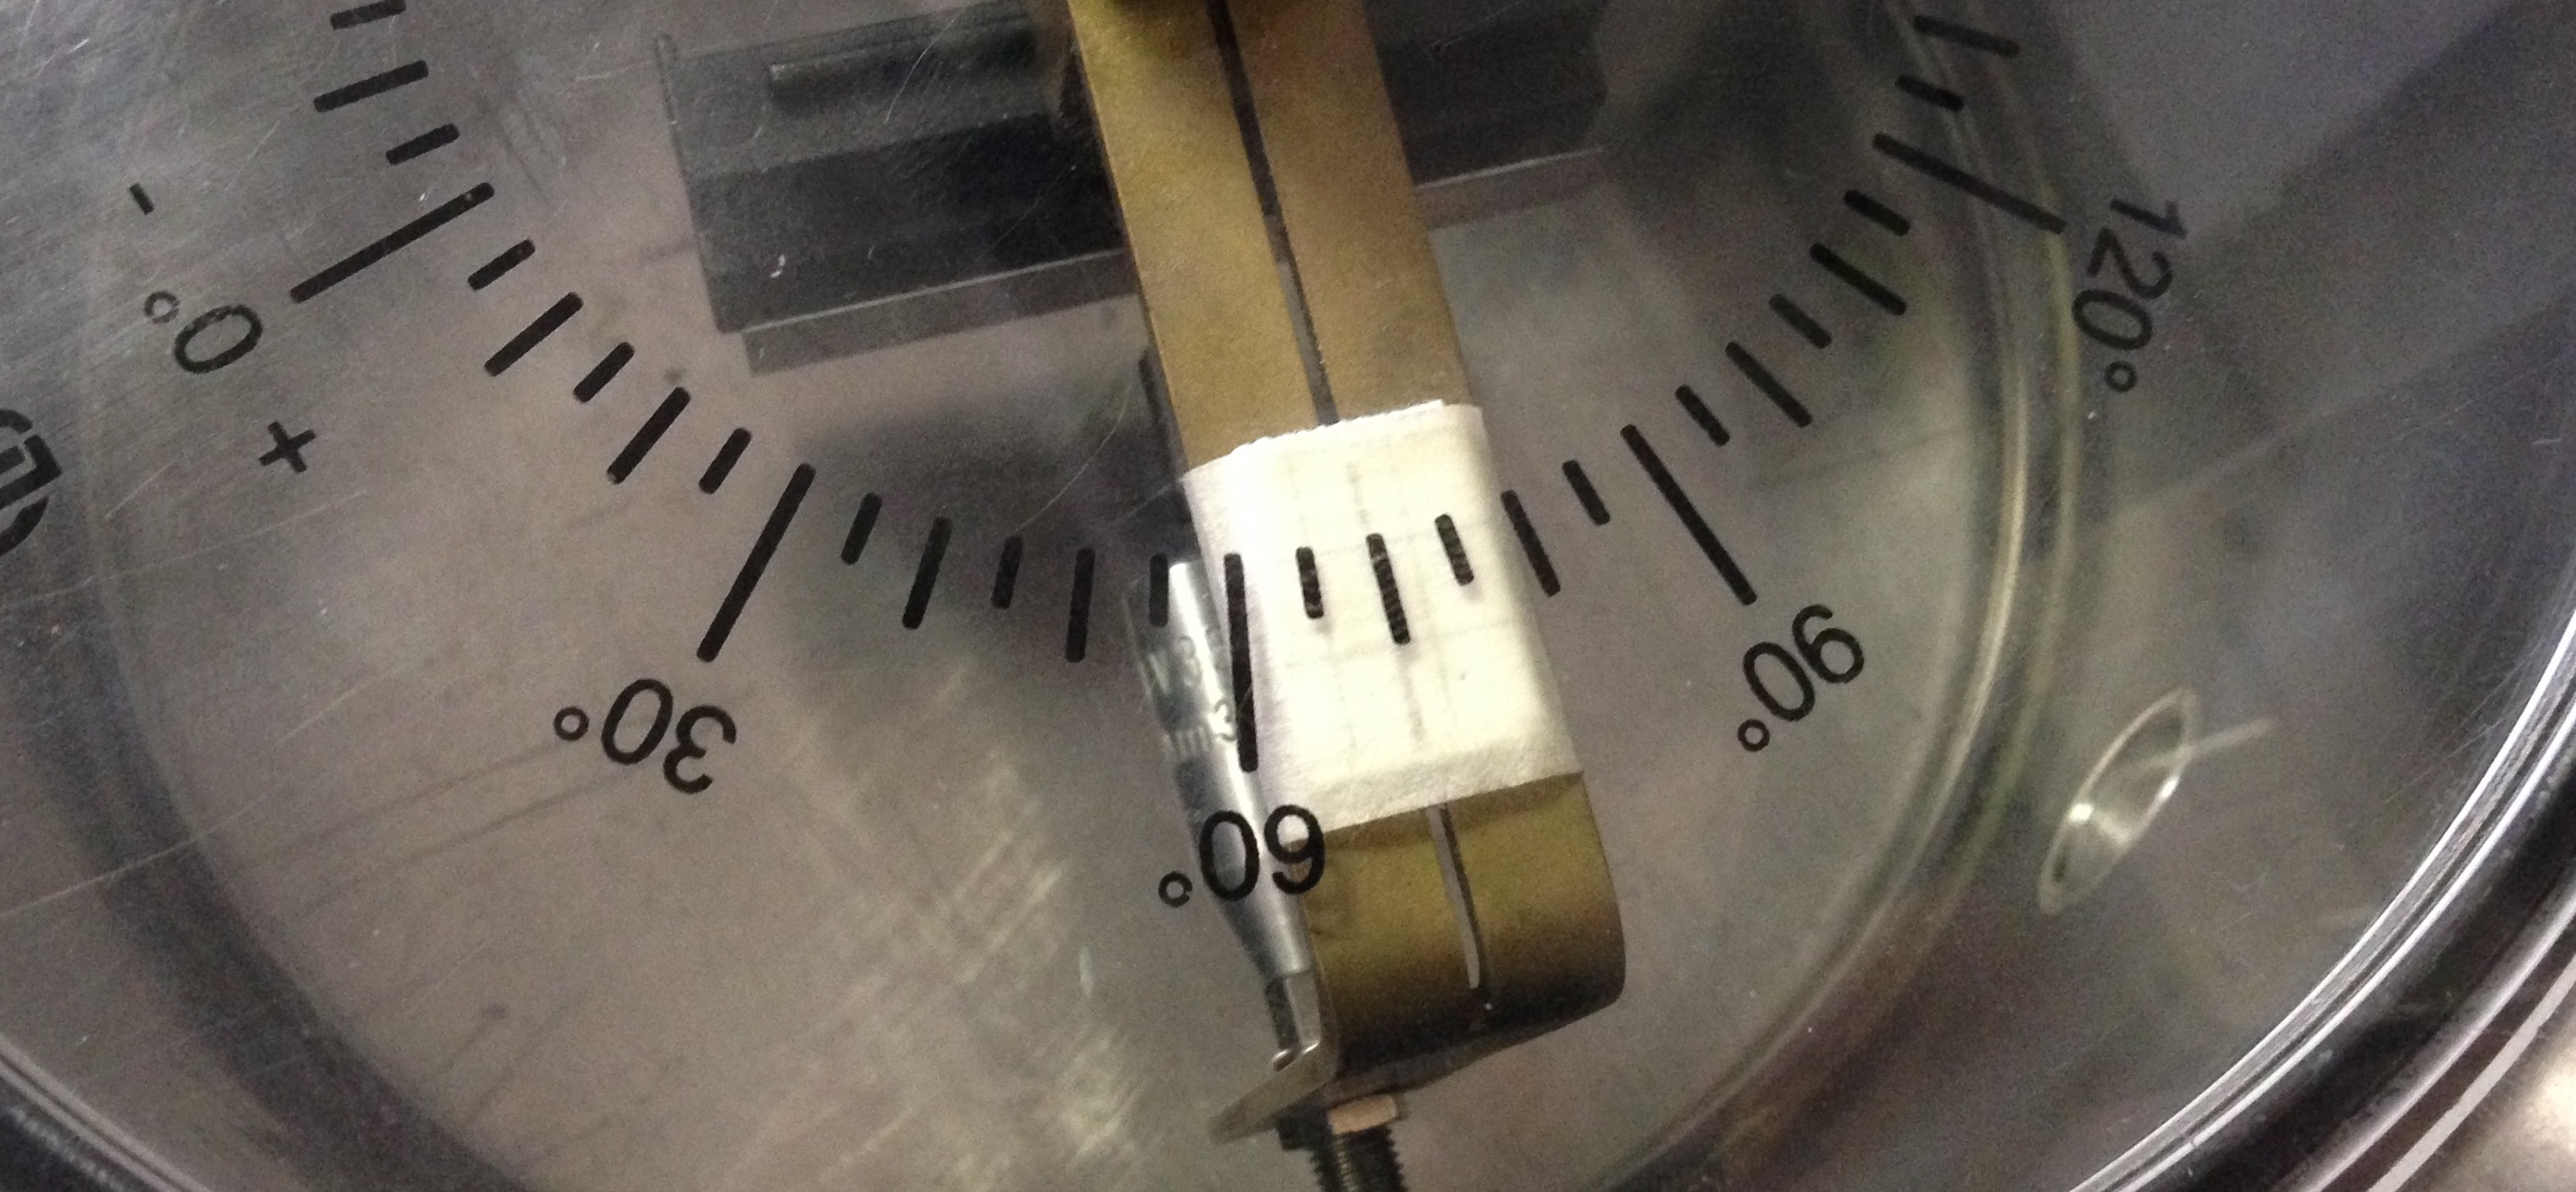
\includegraphics[width=0.6\textwidth]{immagini/parallasse}
	\caption{\label{fig:parallasse}
	Spessore con tacca usato per eliminare la parallasse nella lettura degli angoli.}
\end{figure}

% \paragraph{Energia}
% Per acquisire al meglio i segnali amplificati dobbiamo costruire un circuito che sincronizzi il contatore e l'ADC all'inizio e alla fine di ogni acquisizione.
% Vogliamo comandare l'inizio e la fine di ogni acquisizione agendo sulla levetta di un timer.
% I conteggi vengono effettuati collegando l'uscita TTL del discriminatore ad un generatore di impulsi non retriggerabile, la cui uscita va ad un contatore. Per far partire e fermare un'acquisizione elettronicamente è sufficiente collegare l'uscita del timer allo \emph{start} del contatore e l'\emph{end marker} allo \emph{stop}.
% Per fare la stessa cosa con l'ADC colleghiamo l'uscita del timer (con durata impostata su $\infty$) ad un modulo di coincidenze a cui è connessa, ad un altro ingresso, l'uscita TTL del generatore di impulsi convertita in NIM. Il segnale di coincidenza (convertito in TTL) sarà il trigger dell'ADC, che deve arrivare all'omonimo ingresso \SI{1}{\micro s} prima del segnale affinché ne selezioni il picco.
% Concludiamo la procedura inserendo i ritardi opportuni.

\paragraph{Input ADC}

Evitiamo che segnali superiori a \SI{3.3}{V} danneggino l'ADC ponendo un attenuatore da \SI{0.9}{dB} all'uscita dell'amplificatore.

\paragraph{Interruzioni di corrente}

Quando il crate viene acceso il timer si triggera e avvia la catena di acquisizione.
Questo è utile se la corrente dovesse mancare mentre non siamo presenti.
L'ADC anche se non è connesso al computer salva i dati in un buffer interno di circa 1500 slot,
dal quale possono essere recuperati in seguito.

\subsection{Taratura trigger ADC}

Il ritardo del trigger dell'ADC
rispetto al fronte di salita del segnale discriminato
è stato tarato ponendo la sorgente a \SI{0}{\degree} senza bersaglio
e cercando di massimizzare la lettura del segnale,
in quanto l'output dell'amplificatore ha una forma a campana
con ampiezza proporzionale all'energia in ingresso.
La durata dell'amplificatore è impostata al massimo (\SI6{\micro s}).
Abbiamo acquisito lo spettro a vari angoli e verificato che non dipende dall'angolo in assenza di bersaglio. 
% \marginpar{il fit e la figura sono degli scalda posto per sapere come verrà in seguito}
% Abbiamo fittato lo spettro a \SI{0}{\degree} con una Gaussiana lasciandone libera anche la normalizzazione.\\
% Abbiamo ottenuto:
% \begin{align*}
% \mu &=3115\pm2 \\
% \sigma &= 87\pm2 \\
% N &=(1.18\pm0.02)\cdot10^5 \\
% \chi^2 &=2313\pm15 \\
% \text{dof} &=15 \\
% \end{align*}
% Il valore elevato del $\chi^2$ mostra chiaramente la non gaussianità del picco osservato.

% \begin{figure}[h]
% \centering
% 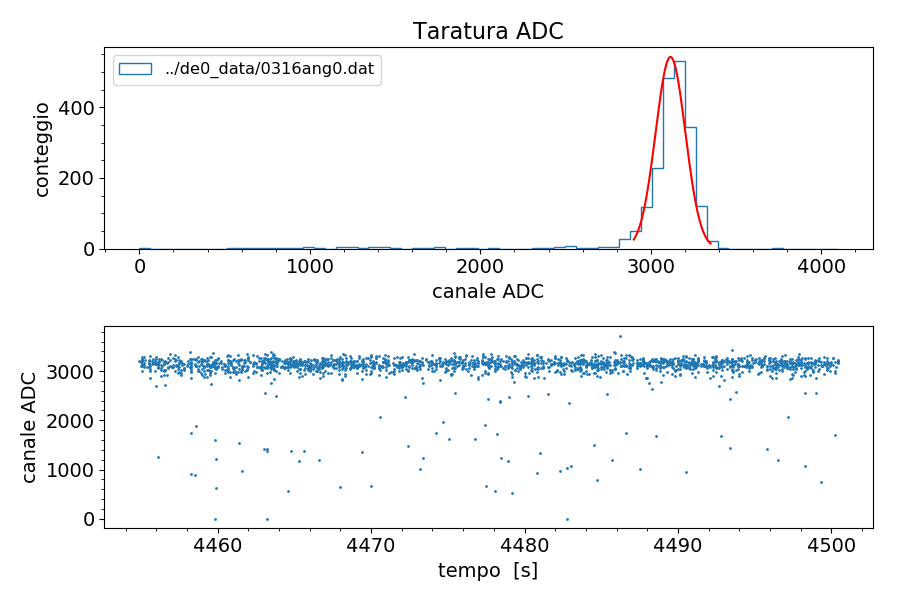
\includegraphics[width=23 em]{immagini/cal_provv}
% \caption{Risoluzione in energia dell'ADC. Il pannello superiore mostra l'istogramma dei dati acquisiti con la funzione di fit, quello inferiore mostra il loro valore in funzione del tempo.}
% \label{tara}
% \end{figure}